





\chapter{Introduction}

As more and more systems are growing using existing P2P technology, we are building services usable by the public (and exploring even more possibilities) based on a P2P system called a Distributed Hash Table.
While current Distributed Hash Tables are an incredible effective and robust solution to maintain a shared state in a P2P system in a scalable fashion, little to no improvement has been provided over the initial Chord\cite{chord} and Kademlia\cite{kademlia} DHTs.
This dissertation explores improvements and applications of Distributed Hash Tables to provide the capacity for future robust and distributed systems infrastructures and services.

\section{The Ship of Theseus}

\singlespacing
\blockquote{The ship wherein Theseus and the youth of Athens returned from Crete had thirty oars, and was preserved by the Athenians down even to the time of Demetrius Phalereus, for they took away the old planks as they decayed, putting in new and stronger timber in their places, in so much that this ship became a standing example among the philosophers, for the logical question of things that grow; one side holding that the ship remained the same, and the other contending that it was not the same.

-Plutarch, Theseus

}
\doublespacing

What has attracted my design and applications of Distributed Hash Tables is that they encourage thinking on a global (or larger) scale and require designs that operate with minimal human intervention on time scales beyond those normally considered by computer science.

In traditional engineering and design we conceive of an object, that while having parts replaced in the course of maintenance, will largely remain a single static object comprised of the same material of which it was formed until it is disposed of.
When considering a Distributed Hash Table, we are intentionally designing a system like the Ship of Theseus, where on the scale of millions of devices are added and lost on a daily basis, often amounting to up to half of the constituent parts of a globe spanning system being replaced in a day.
It is our task to design a pattern of behavior for each of these parts that allows the system to respond to queries despite constant in-progress failure and replacement and to constantly propagate the information stored in the system onward to new storage before the current storage fails. 

Despite the challenge involved in building such a system, barring dramatic change to our expectations of the future, the existing Distributed Hash Tables will be able to persist as a public utility indefinitely.
I present that the answer to the Paradox of the Ship of Theseus is, "I don't care as long as the ship still floats".

\section{Goals}

The goals of the papers making up this dissertation are straightforward.
Four subjects concerning DHTs are open and meriting improvement, generalization, application, efficiency, and robustness. 
\begin{itemize}

\item DGVH and UrDHT present ideas to generalize our model of "What is a Distributed Hash Table" beyond the current proposed methods into a continuum of viable DHT methods which we can explore for ideal properties. 

\item ChordReduce is concerned with application of a DHT to act as an organizing mechanism for a traditional distributed computing paradigm, but with viability at larger scales of operation and duration.

\item Hyperbolic DHTs utilize the generalized model of distributed hash tables to realize the idea of using a hyperbolic coordinate space to improve DHT efficiency that has existed in theory for about a decade.

\item New replication strategies will allow DHTs to store records with essentially zero loss on any time scale the implementers deem appropriate for their uses. 


\end{itemize}



\chapter{Technical Background}
\section{What is a DHT?}
At the core of maintaining a distributed system is establishing a shared state in the form of a table of key-value pairs.
DHTs provide a mechanism for agreeing upon a very large shared state with tolerable inconsistency (records are sometimes lost, and if mutable they may be inconsistent in value).
While other techniques of concensus provide higher confidance, DHTs scale to awesome levels of storage capacity because they are highly tolerant of the failure of nodes within themselves.
In practice, DHTs and similar distributed system's performance are bound by the CAP Theorem\cite{brewer2010certain}.

\subsection{CAP Theorem/ Brewer’s Theorem}
CAP Theorem describes a trade-off between three Attributes of distributed systems.
It states, that any distributed system is a compromise between consistency, availability and partition tolerance and that no distributed store of state can posses all of these qualities at a time.
\begin{itemize}
\item Consistency: Everybody agrees on the contents of shared data
\item Availability: Everybody can quickly and consistently access all the data.
\item Partition Tolerance: The network can handle loss of nodes and connectivity between nodes without loosing the system's cohesion or data.
\end{itemize}

As partition tolerance is required in a DHT for long term operation, this leaves us a trade-off between Consistency and Availability.
In DHTs consistency is limited to assure availability of records to users, however such trade-offs are not binary, and we can can seek a balance between availability and consistency to best suit the needs of applications.


\section{What are the currently existing DHTs?}

Chord and Kademlia are the most commonly used DHTs in practice. 
Chord has been favored by researchers because it was designed with a series of proofs to show its consistency in the face of churn.
Sadly these proofs have been shown to be incorrect\cite{} without serious modification to the established protocol.


\subsection{Chord}
Chord\cite{chord} is a peer-to-peer (P2P) protocol for file sharing and distributed storage that guarantees a high probability $\log_{2} N$ lookup time for a particular node or file in the network. 
It is highly fault-tolerant to node failures and churn, the constant joining and leaving of nodes.  It scales extremely well and the network requires little maintenance to handle individual nodes.  
Files in the network are distributed evenly among its members.

As a distributed hash table (DHT), each member of the network and the data stored on the network is mapped to a unique $m$-bit key or ID, corresponding to one of  $2^m$ locations on a ring. 
The ID of a node and the node itself are referred to interchangeably.

In a traditional Chord network, all messages travel in one direction - upstream, hopping from one node to another with a greater ID until it wraps around.
A node in the network is responsible for all the data with keys \textit{above or upstream} his predecessor, up through and including its own ID.  If a node is responsible for some key, it is referred to being the successor of that key.

Robustness in the network is accomplished by having nodes backup their contents to their $s$ (often 1) immediate successors, the closest nodes upstream.  
This is done because when a node leaves the or fail, the most immediate successor would be responsible for the content its content.

Each node maintains a table of $m$ shortcuts to other peers, called the finger table.   The $i$th entry of a node $n$'s finger table corresponds to the node that is the successor of the key $n+2^{i-1} \mod 2^m $.  Nodes route messages to the finger that is closest to the sought key without going past it, until it is received by the responsible node.  This provides Chord with a highly scalable $\log_2(N)$ lookup time for any key\cite{chord}.

As nodes enter and leave the ring, the nodes use their maintenance procedures to guide them into the right place and repair any links with failed nodes.  Full details on Chord's maintenance cycle are beyond the scope of this paper and can be found here\cite{chord}.

\begin{figure}
	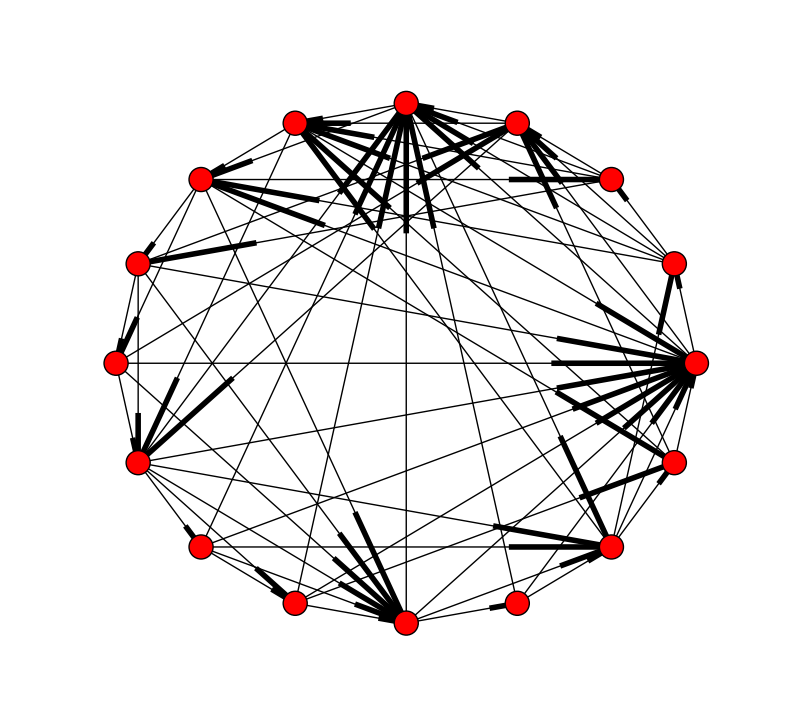
\includegraphics[width=0.5\linewidth]{chordreal}
	\caption{A Chord ring 16 nodes where $m=4$.  The bold lines are incoming edges.  Each node has a connection to its successor, as well as 4 fingers, some of which are duplicates.}
	\label{chordreal}
\end{figure}


\subsection{Kademlia}

Kademlia is the most popular DHT methodology. 
It powers the trackerless bittorent mainline DHT, and the C implementation related to that project is likely the greatest cause of its popularity.
many other distributed systems utilize modified versions of Kademlia as a means of peer management and as a key-value store.

Kademlia is built in a non-eucldian metric space. 
Locations are represented by a large integer (160 bit is most common) and the distance between locations is calculated by the XOR metric.
This means Kademlia's metric space is a generalization of a binary tree, where the locations are mapped to leaf nodes and distance between nodes is the distance required to traverse between them on that tree.

Because of the geometric awkwardness of its metric, Kademlia uses a modified k-nearest neighbors approach to approximate node's voronoi regions and Delaney peers.
If nodes are evenly distributed through the space, kademlia's metric provides an $O(log(n))$ diameter network.


\section{What are DHTs used for}

DHTs are designed to be used to store data in a distributed system that would normally be centrally stored in other systems, like a database or other records.
In practice, they also double as a mechanism for peers discovery and network management.
Many p2p services use a DHT as part of their infrastructure: Bitorrent\cite{jimenez2011kademlia}, CJDNS\cite{hodson2013meshnet}, and I2P\cite{zantout2011i2p}
% %Give examples of how DHTs are used in those projects
